\documentclass{beamer}


\usetheme{CambridgeUS}
\usepackage{graphicx}
\usepackage{float}
\usepackage{ragged2e}
\usepackage{hyperref}
\usepackage{color}
\usepackage{subcaption}

\definecolor{orange}{rgb}{0.93,0.07,0}


\title[Multiphase SPH]{\textbf{Simulation of Multiphase Flows using Smoothed Particle Hydrodynamics(SPH)}\\[0.1in]
		Dual Degree Project - I\\
		\textbf{AE 593}}

\author[Vikas K]{Vikas Kurapati \\ 
		\textbf{Roll no:} 130010058 \\
		Department of Aerospace Engineering\\
		\textbf{I.I.T. Bombay}\\[0.1in]
		\textbf{Guide:} Prof. Prabhu Ramachandran}

\date{October 24, 2017}

\begin{document}

\begin{frame}
\maketitle
\end{frame}

\section{Introduction}

\begin{frame}{Introduction}
\justifying
The current project involves simulation of multiphase flows using Smoothed Particle Hydrodynamics(SPH).\\[0.2in] 
First we discuss formulation of surface tension in multiphase flows and then break down the three forces in Multiphase flows i.e., Pressure, viscous and surface tension forces.\\[0.2in] 
Later, different SPH formulations of surface tension are discussed a method is implemented using PySPH and the results are discussed.
\end{frame}

\section{Basics of SPH Formulations}
\begin{frame}{Basics of SPH Formulations}
\justifying
Any function and its gradient can be interpolated as the follows in SPH:
\begin{eqnarray*}
F_s (r) = \sum_{j} F_j \frac{m_j}{\rho_j} W(r-r_j, h) \\
\nabla F(r) = \sum_j \frac{m_j}{\rho_j}F_j \nabla W(r-r_j, h)
\end{eqnarray*}
\end{frame}
\section{SPH formulations of basic Navier Stokes Equations}
\subsection{Continuity Equation}
\begin{frame}{SPH formulations of basic Navier Stokes Equations}
\begin{itemize}
\item Continuity Equation
\end{itemize}
Continuity Equation gives the evolution of density. The formulations
are as given below:

\begin{equation*}
 \rho_i = \sum_j m_j W_{ij}
 \label{summation}
\end{equation*}

This form of equation for density is called the Summation Density

\noindent
Density can also be evolved by using $\frac{d\rho}{dt} + \rho \nabla . \mathbf{v} = 0$

\begin{equation*}
 \frac{d\rho_i}{dt} = \sum_j m_j \mathbf{v_{ij}} \nabla_i W_{ij}
  \label{Continuity}
 \end{equation*}

where $\mathbf{v_{ij}} = \mathbf{v_i} - \mathbf{v_j}$.\\
\end{frame}

\subsection{Momentum Equation}
\begin{frame}{Momentum Equation}
The pressure forces are approximated as:
\begin{equation*}
 \frac{d\mathbf{v_i^p}}{dt} = -\sum_j m_j \left( \frac{P_j}{\rho_j^2} + \frac{P_i}{\rho_i^2}\right)\nabla_i W_{ij}
\end{equation*}
The commonly used viscous forces in SPH is:
\begin{equation*}
 \frac{d\mathbf{v_i^\nu}}{dt} = - \sum_j m_j \Pi_{ij} \nabla_i W_{ij}
\end{equation*}
where:
\begin{equation*}
 \Pi_{ij} = -\nu \left( \frac{min(\mathbf{v_{ij}}, \mathbf{x_{ij}}, 0)}{(\mathbf{x_{ij}}^2 + \epsilon h_{ij}^2)}\right), 
  \label{pi}
 \end{equation*}
where:
\begin{equation*}
 \nu = \frac{\alpha h_{ij}c_s}{\rho_{ij}}
\end{equation*}
where $\alpha$ is the viscosity constant, $c_s$ is the artificial speed of sound.
\end{frame}

\subsection{Energy Equation}
\begin{frame}{Energy Equation}
The equation for the rate of change of thermal energy per unit mass is given by:

\begin{eqnarray*}
 \frac{du}{dt} = -\left( \frac{P}{\rho} \right)\nabla. \mathbf{v} \\
 \frac{du}{dt} = -\nabla\left(\frac{P\mathbf{v}}{\rho}\right) + \mathbf{v}.\nabla\left(\frac{P}{\rho}\right)
 \end{eqnarray*}

\noindent
By taking the average of the SPH representations of the above:

\begin{equation*}
 \frac{du_i}{dt} = \frac{1}{2} \sum_j m_j \left( \frac{P_j}{\rho_j^2} + \frac{P_i}{\rho_j^2}\right)\mathbf{v_{ij}}.\nabla_i W_{ij}
\end{equation*}

\noindent
note that this has symmetric factors.

\end{frame}

\subsection{Moving The Particles}
\begin{frame}{Moving The Particles}
Particles are moved in the following way with an extra term added called XSPH correction:

\begin{equation*}
\frac{d\mathbf{r_i}}{dt} = \hat {\mathbf{v_i}} = \mathbf{v_i} + \epsilon \sum_j m_j \left(\frac{\mathbf{v_{ji}}}{\rho_{ij}}\right) W_{ij}
\end{equation*}

\noindent
where $\rho_{ij} = 0.5*(\rho_i + \rho_j)$ and $\epsilon (0 \leq \epsilon \leq 1)$ is a tunable constant. 
\end{frame}


\subsection{Equation of State}
\begin{frame}{Equation of State}
\justifying
To close the system of Equations, we need an equation of state which evaluates Pressure.\\
A numerical speed of sound
$c_0 = \sqrt{\left(\frac{dP}{d\rho}\right)_s}$ is used in the EOS.\\

The Suitable equation as given by Tait is given by :

\begin{equation*}
 \Delta P = \frac{c_0^2 \rho_0}{\gamma} \left[ \left( \frac{\rho}{\rho_0} \right)^{\gamma} - 1 \right]
\end{equation*}

\noindent
Using this equation, the pressure can be computed and used in the momentum equations.
\end{frame}

\section{Physics of Multiphase Flows}
\begin{frame}{Physical Foundations of Multiphase Flows}
We will need to track the interface curvature accurately to formulate the surface forces in Multiphase flows
\subsection{Interface Tracking techniques}
In case of immiscible fluids, a property called color can be assigned to them and their tracking can be done by advecting that color function.

\begin{equation*}
\frac{\partial c}{\partial t} + \mathbf{v}.\nabla c = 0 
\end{equation*}

This property is assigned to particles in SPH and their tracking is done to track the interfacial curvature.
\end{frame}

\subsection{Continuum Surface Force Method(CSF)}
\begin{frame}{Continuum Surface Force Method}
\justifying
The Continuum Surface Force Method is used to numerically simulate the surface tension in this work. In CSF model, surface tension is written as a force per unit volume $\mathbf{F_s}$
as:
\begin{equation*}
 \mathbf{F_s} = \mathbf{f_s} \delta_s
\end{equation*}

\noindent
where $\delta_s$ is a normalized surface delta function and $\mathbf{f_s}$ is the force per unit area given by

\begin{equation*}
 \mathbf{f_s} = \sigma \kappa \mathbf{\hat{n}} + \nabla_s \sigma
 \label{forceperarea}
\end{equation*}

\noindent
where $\sigma$ is the surface tension coefficient, $\mathbf{\hat{n}}$ is the unit normal to the interface, $\kappa$ is the curvature to the interface 
and $\nabla_s$ is the surface gradient. The normal can be obtained using
\begin{equation*}
 \mathbf{n} = \frac{\nabla c}{[c]}
\end{equation*}
\noindent
where c is the color function identifying each fluid in the simultion and [c] is the jump in c across the interface. 
\end{frame}

\begin{frame}
The curvature can be calculated as
\begin{equation*}
 \kappa = \nabla . \mathbf{\hat{n}}
\end{equation*}
\noindent
The surface delta function employed in this work is
\begin{equation*}
 \delta_s = \left| \mathbf{n} \right |
\end{equation*}

The second term of the surface tension force where there is a gradient of surface tension coefficient is neglected as only constant surface tension cases are dealt here.
\end{frame}

\section{SPH Formulations}
\subsection{Density}
\begin{frame}{SPH Formulations of Multiphase Flows}
Density is evaluated for every particle at the beginning of the time step using the following equation called as Summation Density. 

\begin{equation*}
 \rho_a = \sum_b m_b W_{ab}
\end{equation*}

\noindent
where $W_{ab}$ denotes

\begin{equation*}
 W_{ab} = W(\mathbf{r_{ab}}, h)
\end{equation*}

\noindent
and

\begin{equation*}
 \mathbf{r_{ab}} = \mathbf{r_a} - \mathbf{r_b}
\end{equation*}
\noindent
where $\mathbf{r_a}$ denotes the position of particle a.
The smoothing length is generally between 1-1.5 times the shortest particle separation. 
\end{frame}

\subsection{Equation of State}
\begin{frame}{Equation of State}
\justifying
For this work, the isothermal EOS as follows is used.

\begin{equation*}
 p_a = c_s^2 (\rho_a - \rho_0)
\end{equation*}

\noindent
where $\rho_0$ is the reference density of the fluid and $c_s$ is the artificial speed of sound. 
Subtracting the reference density was found to lead to more accurate simulations. 
The reason for this is that subtracting the reference density removes a zeroth-order term associated with conservative forms of SPH pressure gradients. 
The speed of sound is chosen to be generally 10 times the maximum velocity of the particles.
\end{frame}

\subsection{Forces: Pressure}
\begin{frame}{Forces: Pressure}
\justifying
The three main forces are pressure, viscous and surface tension forces. \\
\noindent
SPH form of pressure force used in this work is:
\begin{equation*}
 -\left( \frac{1}{\rho} \nabla p\right)_a = -\sum_b m_b \left( \frac{p_a + p_b}{\rho_a \rho_b}\right) \nabla_a W_{ab}
\end{equation*}
\noindent
where $p_a$ is the pressure at particle a and $\nabla_a$ denotes the gradient with respect to the co-ordinates of particle a. 
This form of pressure gradient conserves momentum exactly, since forces acting between individual particles are antisymmetric.
\end{frame}

\subsection{Forces: Viscous}
\begin{frame}{Forces: Viscous}
\justifying
Viscous forces were calculated using a formulation recently applied to low Reynolds Number flow. \\
The SPH momentum equation may be written as:

\begin{equation*}
 \left(\frac{d\mathbf{v_v}}{dt} \right)_a = \sum_b \frac{m_b(\nu_a + \nu_b)\mathbf{v_{ab}}}{\rho_a\rho_b} \left(\frac{1}{r_{ab}} \frac{\partial W_{ab}}{\partial r_a}\right) 
\end{equation*}
\end{frame}

\subsection{Forces: Surface Tension Forces}
\begin{frame}{Surface Tension}
\begin{itemize}
 \item Calculating the Interfacial curvature
\end{itemize}

In order to obtain the surface tension forces, the curvature $\kappa$ should be calculated. 
This requires calculation of surface normals and their divergence.\\

The simplest SPH expression for \textbf{n} is given by
\begin{equation*}
 \mathbf{n_a} = \sum_b \frac{m_b}{\rho_b} c_b^i \nabla_a W_{ab}
\end{equation*}
\noindent
where $c_b^i$ is the color index of particle b. \\
More accurace estimates of the surface normal are obtained when the color field is smoothed by convolution with the kernel. With SPH, this smoothing is done using SPH approximation of the color function.
\begin{equation*}
 c_a = \sum_b \frac{m_b}{\rho_b}c_b^i W_{ab}
\end{equation*}
\end{frame}

\subsection{Calculating Interfacial Curvature}
\begin{frame}
Additional improvements in normals is done using:
\begin{equation*}
 \mathbf{n_a} = \sum_b \frac{m_b}{\rho_b} (c_b - c_a)\nabla_a W_{ab}
  \label{normal}
 \end{equation*}

The simplest SPH expression for the divergence of $\mathbf{\hat n}$ is:

\begin{equation*}
 \left( \nabla . \mathbf{\hat n}\right)_a = \sum_b \frac{m_b}{\rho_b} \mathbf{\hat n_b}.\nabla_a W_{ab}
\end{equation*}
\noindent
A more accurate estimation of divergence is obtained using

\begin{equation*}
 \left( \nabla . \mathbf{\hat n_a}\right) = \sum_b \frac{m_b}{\rho_b}(\mathbf{\hat n_b} - \mathbf{\hat n_a}). \nabla_a W_{ab} 
  \label{divergence}
 \end{equation*}


If the above two equations are used to evaluate the curvature, large errors occur at the transition region's edges. 
The main issue is the requirement of normalized normals $\mathbf{\hat n}$. 
Some distance away from the interface, \textbf{n} will be small and may have a random direction. 
So, any curvature using these normals would be inaccurate. 
Hence, for a more accurate calculation, we used only 'reliable' normals to do the divergence calculations. 
\end{frame}

\begin{frame}
The following were used to do it:

\begin{equation*}
 N_a = 
 \begin{cases}
  1, & if \left|\mathbf{n_a}\right| > \epsilon \\
  0, & otherwise
 \end{cases}
  \label{reliablity}
 \end{equation*}
\noindent
and

\begin{equation*}
 \mathbf{\hat n_a} = 
 \begin{cases}
  \frac{\mathbf{n_a}}{\left| \mathbf{n_a} \right|}, & if N_a=1 \\
  0, & otherwise
 \end{cases}
\end{equation*}

\noindent
$\epsilon$ is generally taken to be $\frac{0.01}{h}$ in this work. An intermediate estimate of curvature is done to correct the divergence for absence of some of the normals in the neighbourhood of particle a.

\begin{equation*}
 \left(\nabla. \mathbf{\hat n}\right)^*_a = \sum_b min(N_a, N_b) \frac{m_b}{\rho_b}(\mathbf{\hat n_b} - \mathbf{\hat n_a}). \nabla_a W_{ab}
\end{equation*}
\end{frame}

\begin{frame}
This estimate can be corrected by a factor of $f_a$
\begin{equation*}
 (\nabla . \mathbf{\hat n})_a = \frac{(\nabla . \mathbf{\hat n})_a^*}{f_a}
\end{equation*}
\noindent
where
\begin{equation*}
 f_a = \sum_b min(N_a, N_b) \frac{m_b}{\rho_b} W_{ab}
\end{equation*}

\noindent
reflects the local number density of particles with 'reliable' normals. \\

The surface tension is then calculated as:

\begin{equation*}
 (\mathbf{a_s})_a = -\frac{\sigma_a}{\rho_a}(\nabla.\mathbf{\hat n})_a \mathbf{n_a}
\end{equation*}

\end{frame}


\subsection{Momentum Conserving Form}
\begin{frame}{Momentum Conserving Form}
The method explained above does not guarantee exact conservation of momentum. 
We now discuss one method which conserves momentum. Surface tension force can be expressed as the gradient of the tensor.

\begin{equation*}
 \kappa \mathbf{\hat n} \delta_s = \nabla[(\mathbf{I} - \mathbf{\hat n}\times\mathbf{\hat n})\delta_s]
\end{equation*}

\noindent
The given expression can be approximated in SPH by:

\begin{equation*}
 (\mathbf{a_s})_a = \left( \frac{1}{\rho} \frac{\partial S_{ij}}{\partial x_j} \right) = \sum_b m_b \frac{(S_{ij})_a + (S_{ij})_b}{\rho_a \rho_b} \nabla_{a, j} W_{ab}
\end{equation*}
\noindent
where 
\begin{equation*}
 S_{ij} = \delta_s(\delta_{ij} - \mathbf{\hat n_i}\mathbf{\hat n_j})
\end{equation*}

\noindent
Where, $\delta_{ij}$ is the Kronecker delta, $\nabla_{a,j}W_{ab}$ is the $j^{th}$ component of the gradient of $W_{ab}$ with respect to $\mathbf{r_a}$ and the repitition of j means summation. 
\end{frame}

\begin{frame}
To improve accuracy, only reliable normals are used. Since, the reciprocal particle summations are anti-symmetric, this conserves the momentum.\\

This method is potentially unstable as attractive forces when momentum conserving formulations used are unstable when SPH particles are considered.\\
As the resolution is increased, the maximum of $\delta_s$ will increase and at some point, the method will blow up. 
A solution to this issue is to replace $S_{ij}$ with a modified tensor as follow:

\begin{equation*}
 S_{ij}^* = S_{ij} - \delta_{ij}\times max(\delta_s)
\end{equation*}
\end{frame}

\subsection{Removing the Singularity}
\begin{frame}{Removing the Singularity}
\justifying
A disadvantage of the momentum conserving formulation explained above is that the delta function introduces a singularity in the pressure field as the resolution is increased. 
A work around for this is the following(taking [c] = 1)
\begin{equation*}
 \mathbf{F_s} = \sigma \kappa \nabla c = \nabla(\sigma \kappa c) - \sigma c \nabla \kappa
\label{singular}
 \end{equation*}
\noindent
\begin{equation*}
 p^* = p - \sigma \kappa c
\end{equation*}
\begin{equation*}
 \mathbf{F_s^*} = - \sigma c \nabla \kappa 
 \label{surface}
\end{equation*}
\noindent
So, the same momentum equation will be used replacing surface tension forces and with modified pressure boundary conditions which accommodate the new definition of pressure.\\ 
To improve the stability of this technique, only the curvature of those particles which satisfy $\left | \mathbf{n_a}\right| > \epsilon$ are used in the calculations.\\
\end{frame}

\section{Results and Discussions}
\begin{frame}{Results and Discussions}
The following test case was implemented in PySPH using the method of Interface curvature described in the above sections. \\
\begin{itemize}
 \item Stability of an Interface:
\end{itemize}
Previous studies using the CSF formulation have reported a numerical instability at the fluid-fluid interface. 
Using SPH, these currents could lead to particle disorder at the fluid-fluid interface, showing the effect of the diffusing at the interface. \\

This phenomena is studied here: A simple static case in a periodic domain spanning 0.5 units in x-direction and 1 unit in y-direction with upper half with fluid of color 1 and lower half with fluid of color 0 is simulated. 
The fluid densities were considered constant of 1, the surface tension coefficient to be 1 and inviscid flow is considered. 
The speed of sound for this simulation is set to 20 units. 
At t=0, a constant velocity in both directions is set so as the KE of each particle is 6 orders less than their internal energy. 
\end{frame}

\section{Results}
\subsection{Kernels' Comparisions}
\begin{frame}
\begin{figure}[H]
\centering
\begin{subfigure}[b]{0.33\textwidth}
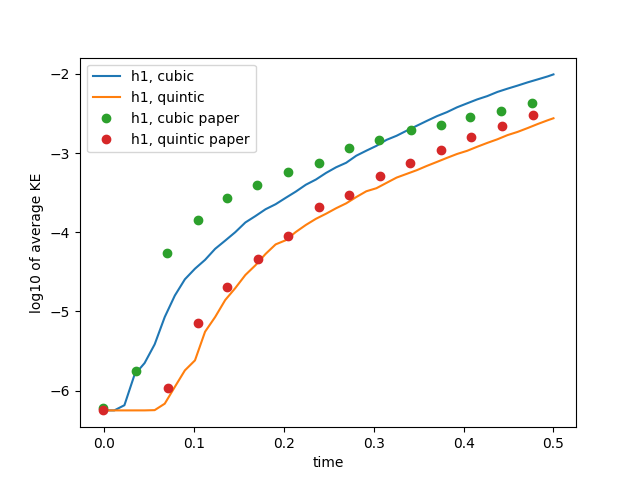
\includegraphics[width=\linewidth]{./case10.png}
\caption{h=h1=1.0}
\end{subfigure}
\begin{subfigure}[b]{0.33\textwidth}
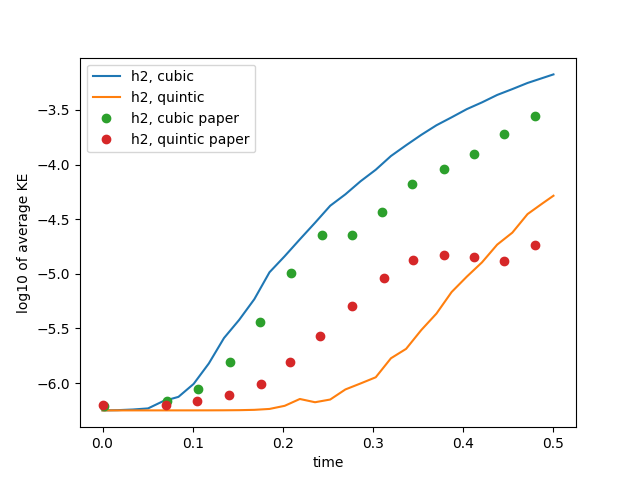
\includegraphics[width=\linewidth]{./case11.png}
\caption{h=h2=1.5}
\end{subfigure}

\begin{subfigure}[b]{0.33\textwidth}
\centering
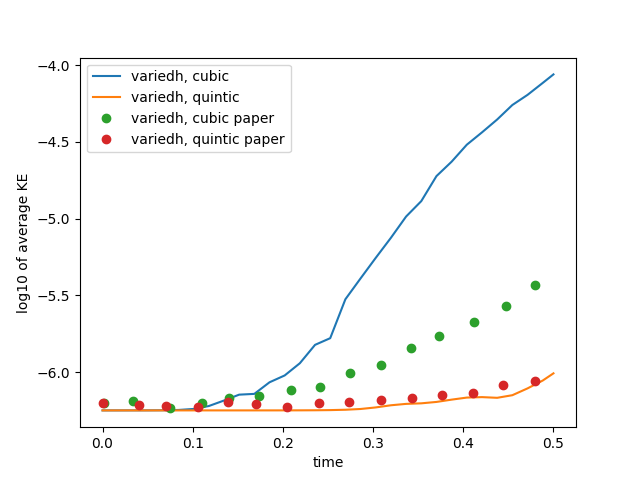
\includegraphics[width=\linewidth]{./case12.png}
\caption{Varied smoothing length}
\end{subfigure}
\caption{Variation of KE for different smoothing lengths}
\end{figure}

In all the cases it can be clearly seen that the Quintic spline has better stability with lower diffusion and KE than the cubic spline. The variations in results when compared to as the initializations used are not exactly random(as it was not explained in the paper, how the initializations were done),
we used a constant velocity in both the dimensions and the magnitude was used so as to match, the initial KE. 
\end{frame}


\subsection{Smoothing Lengths' Comparisions}
\begin{frame}
The following plots show the comparisions of the solutions for different smoothing lengths for various kernels: Cubic spline and Quintic Spline

\begin{figure}[H]
\centering
\begin{subfigure}[b]{0.45\textwidth}
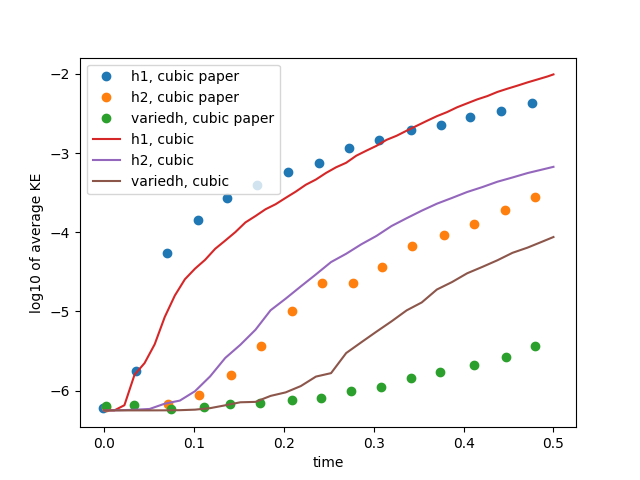
\includegraphics[width=\linewidth]{./case13.png}
\caption{Cubic Spline}
\end{subfigure}
\begin{subfigure}[b]{0.45\textwidth}
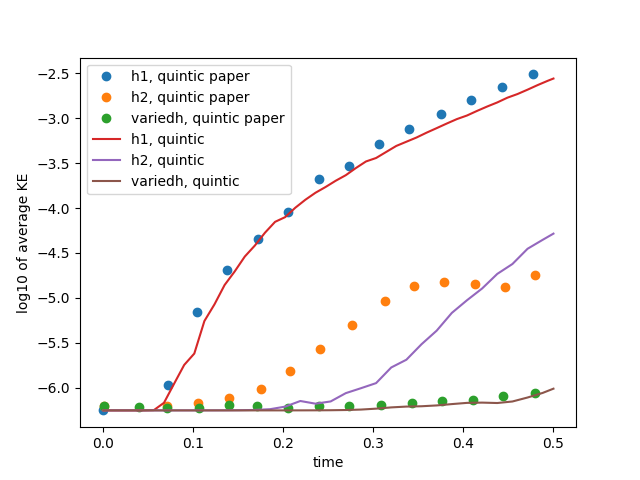
\includegraphics[width=\linewidth]{./case14.png}
\caption{Quintic Spline}
\end{subfigure}
\caption{Variation of KE for different Kernels}
\end{figure}

In all the cases, it can be noted that the varied smoothing lengths when used give the best solution preventing diffusion, then h2=1.5 and h1=1.0 has the worst simulation. 
\end{frame}

\section{Discussions}
\begin{frame}
It can be seen from the plot that the variableh case has better stability of the interface preventing much diffusion of the particles into each other.\\

It is seen that, for the same parameters, the quintic spline is more stable than the cubic spline.\\

Also, the increased smoothing length caused to a considerable amount of stability in the interface. The best stability properties are however exhibited when the smoothing length for curvature is higher than that of delta function calculation.
\end{frame}

\section{Conclusions}
\begin{frame}
 Implementation of surface tension forces in the regime of Smoothed Particle Hydrodynamics(SPH) was discused in this work. 
 Specialized expressions for curvature between two species of particles are formulated. The most straightforward method which calculates the SPH estimate of curvature and applying it directly to get surface tension force is discussed. 
 The issue of not conserving momentum is tackled by a tensor form which might have singularities. 
 A corrected form of pressure and surface tension forces are discussed to tackle that issue.
\end{frame}

\section{Future Work}
\begin{frame}
The following are to be implemented in the second phase of this project:
\begin{itemize}
 \item The already simulated problem using surface tension is to be implemented in the other two methods which were explained using the momentum conserved form and the form 
 which removes the singularities.
 \item Other benchmark problems which include Equilibrium rod, Oscillating rod, Capillary Wave, Three Phase interaction etc.,
 will be implemented using different schemes.
 \item These implementations can be extended to three dimensional problems
 \item A volume density based method where the ratio of mass and density will be replaced
 by the volume of the particle. This implementation will be useful for problems with high density variations.
  \item All these equations put together can be made into a new scheme which can be readily
  used by a user in PySPH.
 \end{itemize}
\end{frame}

\section*{Thank You}
\begin{frame}
\centering
\Huge{\textcolor{orange}{Thank You!}}
\end{frame}

\end{document}
